\item \textbf{{[}DHS/PRELIM/9597/2016/P2/Q1{]} }

GovBuy is a Government Digital Services initiative that helps government
employees buy microservices (small pieces of software that can be
deployed independently), software libraries, non-critical bug fixes
or even customised hardware from independent contractors. 

The platform allows government employees to post a task. Anyone can
bid to take on the task during the bidding period. The reverse auction
starts at \$5,000 and the lowest bid wins.

The winner works on the task and submits completed code to the team.
If the code meets the acceptance criteria before the deadline, the
winner is sent a cheque for the work.

The current prototype platform is a web interface:
\begin{center}
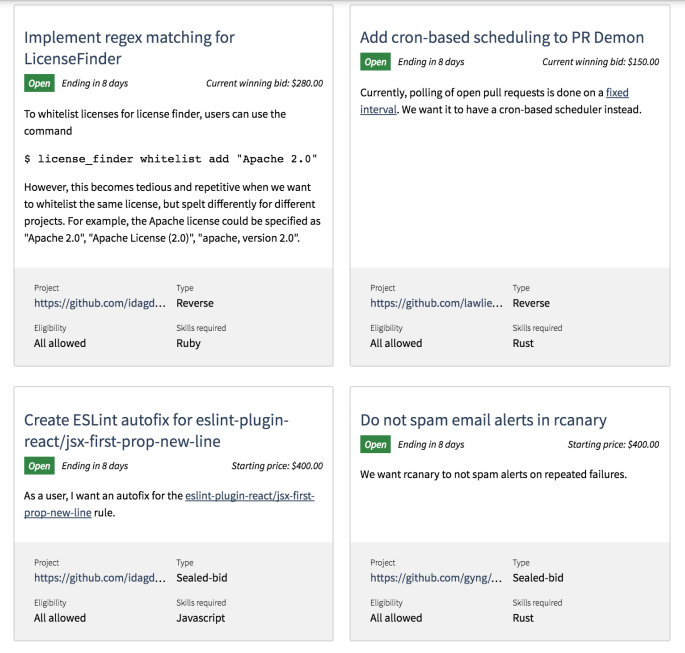
\includegraphics[width=0.5\paperwidth]{C:/Users/Admin/Desktop/Github/question_bank/LyX/static/img/9597-DHS-2016-P2-Q1-1}
\par\end{center}
\begin{enumerate}
\item The agency in charge wishes to develop mobile native versions of the
platform for Android and iOS. The following diagram shows the expected
workflow. 
\begin{center}
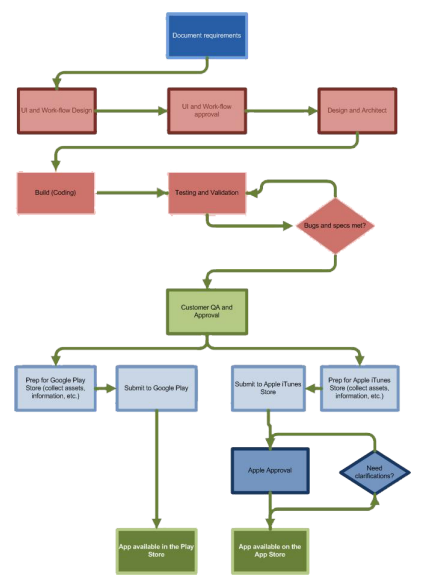
\includegraphics[width=0.5\paperwidth]{C:/Users/Admin/Desktop/Github/question_bank/LyX/static/img/9597-DHS-2016-P2-Q1-2}
\par\end{center}
\begin{enumerate}
\item Create a PERT chart from the above workflow diagram. You may assume
the following durations from the activity table below.\hfill{} {[}4{]}
\noindent \begin{center}
\begin{tabular}{|c|l|c|}
\hline 
Phase & Description & Duration (weeks)\tabularnewline
\hline 
A & Gather and document requirements & 2\tabularnewline
\hline 
B & UI and workflow design and approval & 3\tabularnewline
\hline 
C & Design and architect & 4\tabularnewline
\hline 
D & Build (coding) & 7\tabularnewline
\hline 
E & Testing and validation & 3\tabularnewline
\hline 
F & Customer QA and approval & 2\tabularnewline
\hline 
G & Prepare and submit to Google Play Store & 1\tabularnewline
\hline 
H & Prepare and submit to Apple App Store & 1\tabularnewline
\hline 
I & Apple approval & 1\tabularnewline
\hline 
\end{tabular} 
\par\end{center}
\item From the PERT chart, state the critical path and the minimum project
completion time. \hfill{}{[}2{]}
\item Describe two benefits which can be gained by producing a PERT chart.\hfill{}
{[}2{]}
\item Describe and give an example of a dependent activity. \hfill{}{[}2{]}
\item Describe and give an example of a concurrent activity.\hfill{} {[}2{]}
\end{enumerate}
\item The project manager decides he needs another diagrammatic tool to
monitor the project progress.
\begin{enumerate}
\item Create a Gantt chart for the project.\hfill{} {[}3{]}
\item Explain how the Gantt chart can help the developers in carrying out
their work.\hfill{} {[}2{]}
\end{enumerate}
\item Describe two activities to mark the closure of the project. \hfill{}{[}4{]}
\item Cybersecurity is of paramount concern when it comes to government
web services. Using suitable examples, explain the following cybersecurity
exploits and suggest how they can be mitigated. 
\begin{enumerate}
\item Cross site scripting \hfill{}{[}3{]}
\item Code injection \hfill{}{[}3{]}
\item Denial of service attack \hfill{}{[}3{]}
\end{enumerate}
\item The platform will be hosted using cloud computing. 
\begin{enumerate}
\item Explain why the cloud is a suitable hosting platform. \hfill{}{[}2{]}
\item Use suitable example to illustrate the concepts of IaaS, PaaS and
SaaS. \hfill{}{[}6{]}
\end{enumerate}
\item What ethical considerations should bidders bear in mind when bidding
for tasks on an open source platform such as GitHub?\hfill{} {[}2{]}
\end{enumerate}